\documentclass[letterpaper]{article} 
\usepackage[left = 0.5in, right = 0.5in, top = 0.9in, bottom = 0.9in]{geometry}
\usepackage{enumitem}
\usepackage{multicol}
\usepackage[spanish]{babel}
\usepackage[utf8]{inputenc}

\usepackage{amsmath,amssymb,amsthm}
\usepackage{tikz-cd}
\usepackage{mathrsfs}
\usepackage[bbgreekl]{mathbbol}
\usepackage{dsfont}
\usepackage{graphicx}
\graphicspath{{img/}}

\newcommand{\op}{\operatorname}
\newcommand{\Op}{^{\op{op}}}
\newcommand{\scc}{\mathscr C}
\newcommand{\scd}{\mathscr D}
\newcommand{\sce}{\mathscr E}
\newcommand{\sci}{\mathscr I}
\newcommand{\scj}{\mathscr J}
\newcommand{\scx}{\mathscr X}
\newcommand{\var}{\mathrm{Var}}
\newcommand{\Id}{\operatorname{Id}}
\newcommand{\N}{\mathbb N}
\newcommand{\Z}{\mathbb Z}
\newcommand{\Q}{\mathbb{Q}}
\newcommand{\I}{\mathbb{I}}
\newcommand{\R}{\mathbb{R}}
\newcommand{\C}{\mathbb{C}}
\newcommand{\F}{\mathcal{F}}
\newcommand{\G}{\mathcal{G}}
\newcommand{\B}{\mathcal{B}}
\newcommand{\abs}[1]{\left\lvert #1 \right\rvert}
\newcommand{\inv}{^{-1}}
\renewcommand{\to}{\rightarrow}
\newcommand{\ent}{\Longrightarrow}
\newcommand{\E}{\mathbb{E}}
\renewcommand{\P}{\mathbb{P}}
\newcommand{\1}{\mathds{1}}
\renewcommand{\qedsymbol}{$\blacksquare$}

\theoremstyle{definition}
\newtheorem{dfn}{Definición}
\theoremstyle{definition}
\newtheorem{teo}{Teorema}
\theoremstyle{definition}
\newtheorem{cor}{Corolario}
\theoremstyle{definition}
\newtheorem{prop}{Proposición}
\theoremstyle{definition}
\newtheorem{obs}{Observación}


\title{\textbf{Cómputo Científico\\
Tarea 10\\
Deep neural networks}}
\author{Iván Irving Rosas Domínguez}
\date{\today}

\DeclareSymbolFontAlphabet{\mathbbm}{bbold}
\DeclareSymbolFontAlphabet{\mathbb}{AMSb}
\DeclareMathSymbol\bbDelta  \mathord{bbold}{"01}

\begin{document}
\maketitle

%\begin{abstract}
%\end{abstract}

\begin{itemize}
    \item[\textbf{1.}] Usando la base de datos MNIST realice lo siguiente y explique cada decisión tomada:
    \begin{itemize}
        \item Diseñe una red neuronal de una sola capa oculta para la clasificación de las imágenes. Use una función de 
        pérdida predefinida.\\

        \textbf{Solución:} Utilizando el tutorial que nos fue entregado, creamos una red neuronal para la clasificación de las imágenes 
        de la base MNIST. El diseño que se hizo fue el de una red neuronal con una capa oculta la cual es convolucional, donde el 
        único canal de entrada de 28x28 se transforma en 7 canales de salida utilizando un kernel de $4\times4$. Esto nos da origen a 
        un output de 7 canales de imágenes de $25\times25$. Para la capa de salida, se utiliza una conexión completa con 
        cada una de las 10 posibles clases (correspondientes a cada uno de los 10 números). Para realizar lo anterior, se aplanan los 7 canales de 25$\times$25 para que se tengan las 
        dimensiones adecuadas.\\

        La razón de la elección de las capa anteriores es meramente heurística: las redes neuronales convolucionales intuitivamente
        codifican/procesan mejor las imágenes dada su naturaleza convolutiva.
        En cuanto a la función de activación, se elige la función Relu. La razón de la elección es meramente por desconocimiento de otras funciones, 
        así como también el hecho de que esta función ejecutó un buen trabajo.\\
        
        Se elige un tamaño de batch de 50, dado que el tamaño de la base de datos 
        destinada a entrenar es de 60 000, de tal forma que trabajar los datos con los 'lotes' 
        de tamaño 50 suena razonable.\\

        En cuanto a la función de pérdida, se utiliza la función de entropía cruzada, mientras 
        que el método para optimizar es el descenso de gradiente estocástico. La tasa de aprendizaje se define en 0.001. 
        Nuevamente las elecciones anteriores están motivadas en la prueba de la red y su óptimo desempeño en los resultados.\\

        \item Entrene la red neuronal.\\
        
        \textbf{Solución:} tal como se muestra en el archivo de Google Collab, la red neuronal se entrena utilizando 
        10 épocas. Aproximadamente luego de 3 minutos de entrenamiento utilizando la GPU proporcionada por 
        el servicio, este finaliza. Presentamos brevemente los resultados obtenidos aquí.\\

        Se obtiene que la exactitud de las predicciones de la red es de 97\%, esto es, del total de los 10 000 datos, en el 97\% de ellos coincidió la categoría en 
        la cual la red colocó al dato con la categoría a la cual este mismo dato pertenece. Esto se puede observar en la parte superior de la figura 1.\\
        
        Buscando en qué lugares la red no ejecutó un buen trabajo, se obtienen los resultados de la figura 1. Observamos que el desempeño en la categoría del 9 es el más pobre con 95\% de precisión 
        aproximadamente, mientras que el mejor desempeño lo tiene la categoría del 1 con 99.1\%.
        \begin{figure}[h!]
            \centering
            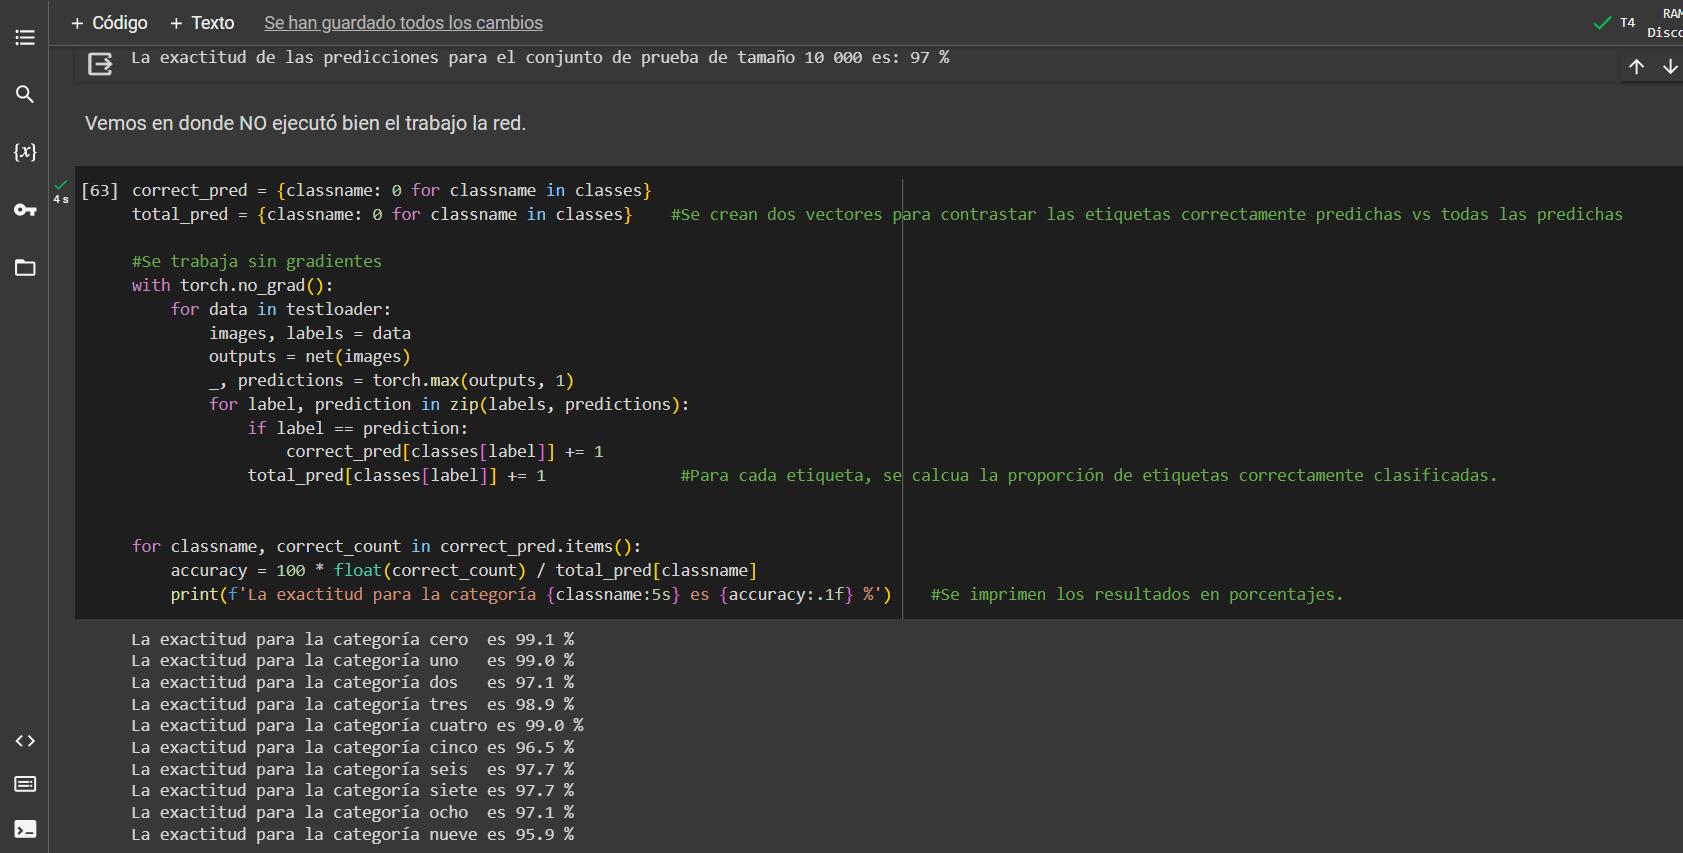
\includegraphics[width=0.6\linewidth]{1.png}
            \caption{Exactitud de la red neuronal en todo el conjunto de datos y la exactitud en cada una de las categorías.}
        \end{figure} 
        \item Presente la matriz de confusión (Confusion matrix).
         Presentamos a continuación la matriz de confusión en la figura 2.
        \begin{figure}[h!]
            \centering
            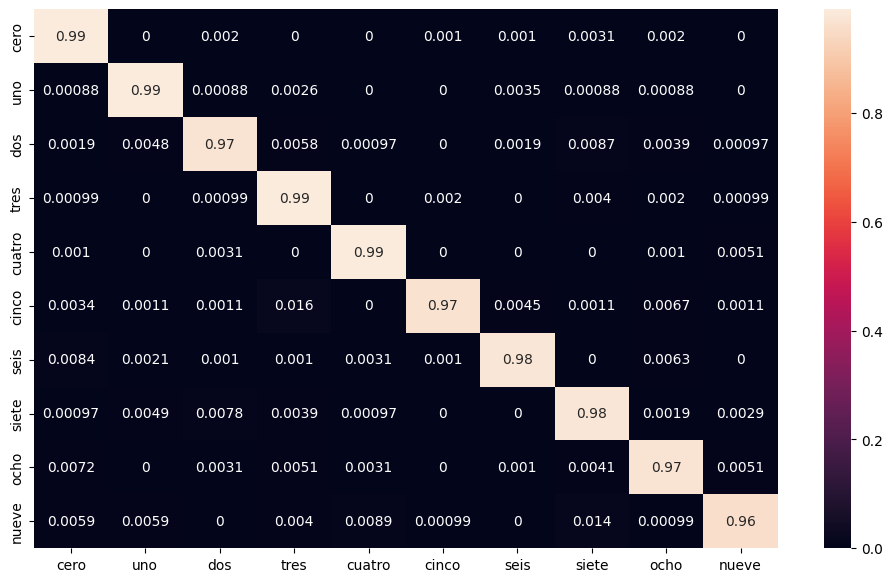
\includegraphics[width=0.8\linewidth]{2.png}
            \caption{Matriz de confusión. El eje x representa los valores predichos. El eje y representa los valores reales.}
        \end{figure} 
        Observamos que hay un excelente comportamiento de la red.  Observamos que hay ceros en la matriz. Es decir, hay valores que la red,
         al momento de hacer la predicción, nunca fueron confundidos como posibles respuestas a la predicción. Por ejemplo, en la predicción del cinco, los números uno, dos, cuatro, 
         siete y ocho nunca fueron confundidos como un cinco por la red.
         \newline
         
         Por otro lado, aunque con un porcentaje bajo, la red otorgó un 1.6\% de sus predicciones del número tres al número cinco, así como otorgó un 1.4\% de sus predicciones 
         del número siete al número nueve. Esto puede interpretarse como que la red 'confundió' con dichos porcentajes al número tres con un número cinco, y al número siete con el número 
         nueve, respectivamente.
        \item Describa que es la precisión y la recuperación (precision and recall) y calcúlelos a partir de su 
        matriz de confusión.\\

        \textbf{Solución:} 
    \begin{itemize}
        \item La \textbf{precisión} (para una clase, digamos, el 'uno' en nuestro caso) está definida como el número total de aciertos que tuvo la red 
        al predecir un dato de tal categoría en el conjunto de prueba, dividido entre el número total de predicciones que fueron hechas para tal categoría. Por ejemplo, la precisión para la 
        categoría 'uno' es el cociente entre la cantidad de aciertos que tuvo la red al predecir datos que verdaderamente eran 'uno', con la cantidad de datos que la red predijo que
        eran el número 'uno'.

        Justamente esta cantidad tiene que ver con qué tan precisa es la red al etiquetar un dato como 'uno'. Por ende, se puede pensar en esta cantidad como una medida de la 
        'confiabilidad' de la red cuando arroja que en efecto un dato pertenece a la categoría 'uno'.
        \item La \textbf{recuperación} (para una clase) está definida como el cociente entre el total de aciertos que tuvo la red al predecir un dato de tal clase, con el conjunto de 
        datos que en efecto forman parte de tal categoría. Por ejemplo, en nuestro caso, la recuperación de la clase 'uno' es la proporción entre la cantidad de veces que la red predijo 
        correctamente un dato como parte de la categoría 'uno', con la cantidad de datos del conjunto de entrenamiento que en efecto eran 'uno'. 
        \newline

        Esta cantidad justo nos indica qué tanto recuperamos una correcta clasificación de los 'uno' que hay en el conjunto de datos. 
    \end{itemize}

    En nuestro caso, tenemos los siguientes datos con respecto la precisión y a la recuperación de nuestra red:
    Presentamos a continuación la matriz de confusión en la figura 2.
    \begin{figure}[h!]
        \centering
        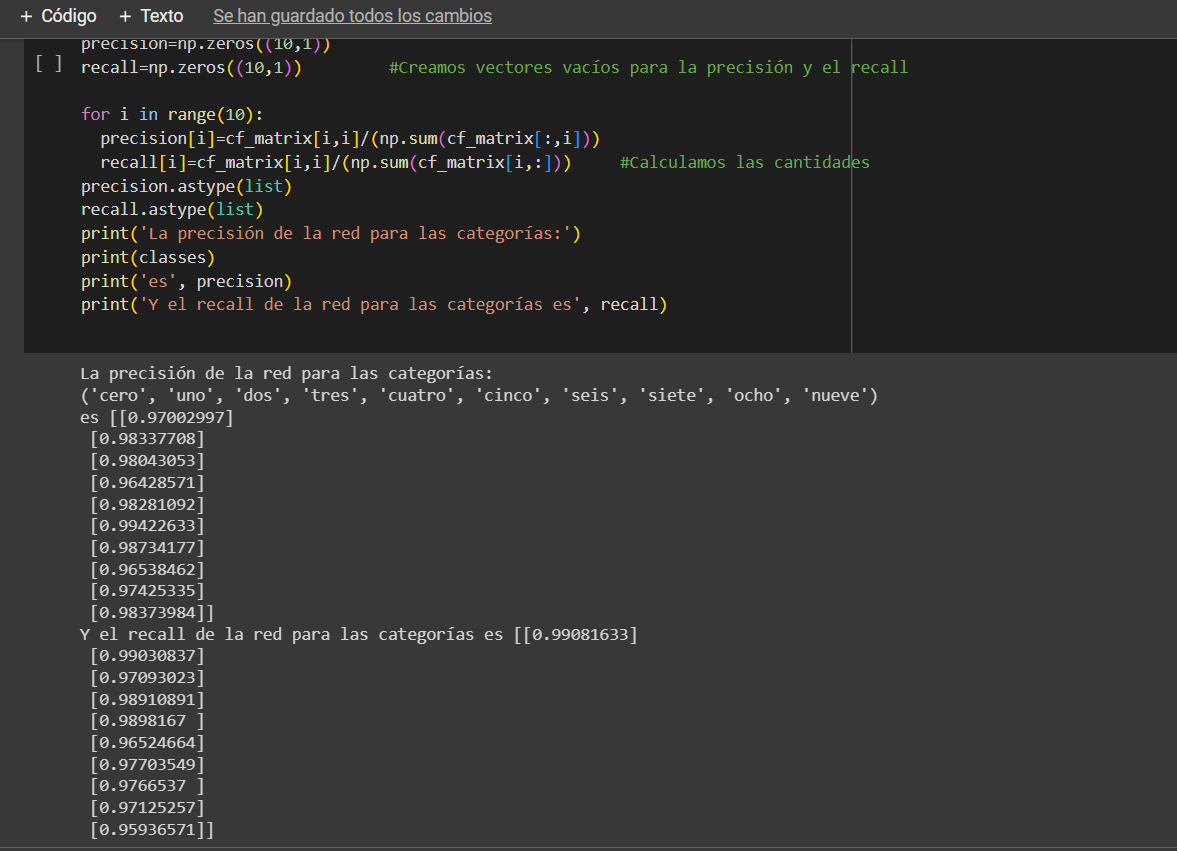
\includegraphics[width=0.8\linewidth]{3.png}
        \caption{Precision y recall para esta red neuronal con esta base de datos.}
    \end{figure} 
    \end{itemize}
    Observamos que ambas medidas son bastante buenas en este conjunto de datos, ya que 
    para cada una de las categorías se obtienen valores entre el 96\% y el 99\%.
\end{itemize}
\end{document}